\documentclass[a4paper]{article}

\usepackage{amsmath, graphicx, float, blindtext} % for dummy text
\graphicspath{ {./images/} }
\title{Chapter 17: Metric Predicted Variable with One Metric Predictor}
\author{Shubham Gupta}

\begin{document}
\maketitle

\section{Introduction}
\begin{itemize}
    \item Scenarios such as predicting weight from height for a person
    \item Predicted variable: metric
    \item Predictor variable: metric
    \item Relationship between $y$ and $x$ will be a linear model with distributed residual radomness in $y$ i.e \textit{simple linear regression} 
    \item Generalize linear regression in 3 ways
        \begin{itemize}
            \item Use t distribution instead of normal distribution to accommodate outliers
            \item Replace linear trend with quadratic trend
            \item Hierachical model to determine individual trend and estimate group level trends as well
        \end{itemize}
        \begin{figure}[H]
            \centering
            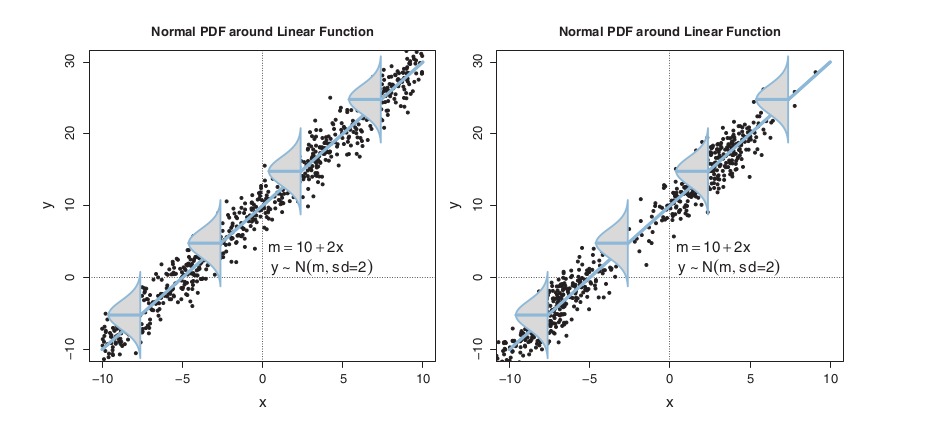
\includegraphics[width=0.8\textwidth]{normal_function}
            \caption{Points for a normally distributed function}
            \label{fig:normal_function}
        \end{figure}
    \item Function: $\mu = \beta_0 + \beta_1x$
    \item Current model only specifies dependency of $y$ on $x$. It does not show how $x$ is generated and no prob dist assumed for $x$.
    \item \textbf{Homogeneity of Variance}: For every value of $x$, the variance in $y$ is te same.  
\end{itemize}
\section{Robust Linear Regression}
\begin{figure}[H]
    \centering
    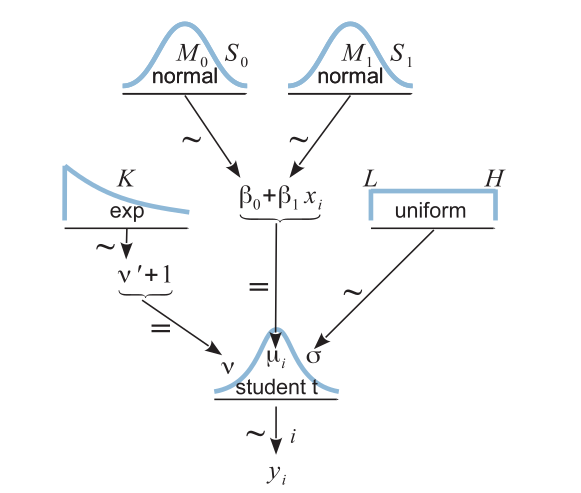
\includegraphics[width=0.8\textwidth]{robust_regression}
    \caption{Robust Linear regression}
    \label{fig:robust_regression}
\end{figure}
\begin{itemize}
    \item $y$ is a t-distribution with mean $\mu$
    \item $\mu$ has $\beta_0$ and $\beta_1$ which are both normal distributions
    \item Scale $\sigma$ is a uniform prior
    \item Normality $\nu$ is an exponential prior
\end{itemize}
\subsection{Standardizing data}
\begin{itemize}
    \item As shown in the figure, there are points where there are many regression lines flowing through them.
    \item These points are a collection of a large number of regression lines.
    \item Sampling from this tightly corelated space can be difficult.
    \item Two ways to make sampling faster:
        \begin{itemize}
            \item Change sampling algo. Instead of Gibbs, use HMC.
            \item Transform regression lines to ensure no strong corelation between slopes and intercepts.
        \end{itemize}
    \item \textbf{Standardize}: Rescaling data relative to mean and SD.  
    \item If input data is standardized, output will also be on a standardized scale. 
\end{itemize}
\subsection{Interpreting posterior distribution}
\begin{itemize}
    \item Model estiamtes are tighter for example with 300 samples.
    \item The graph suggests that there might be positive skew in the dataset.
\end{itemize}
\section{Hierachical regression on Individuals within groups}
\begin{itemize}
    \item We can estimate reression lines for each individual and group if we have data in the form $x_{i|j}l$ and $y_{i|j}$. $i|j$ represents  $i^{th}$ observation for  $j_{th}$ individual.
    \item Goal: Describe each individual with linear regression and estimate group level characteristics.
    \begin{figure}[H]
        \centering
        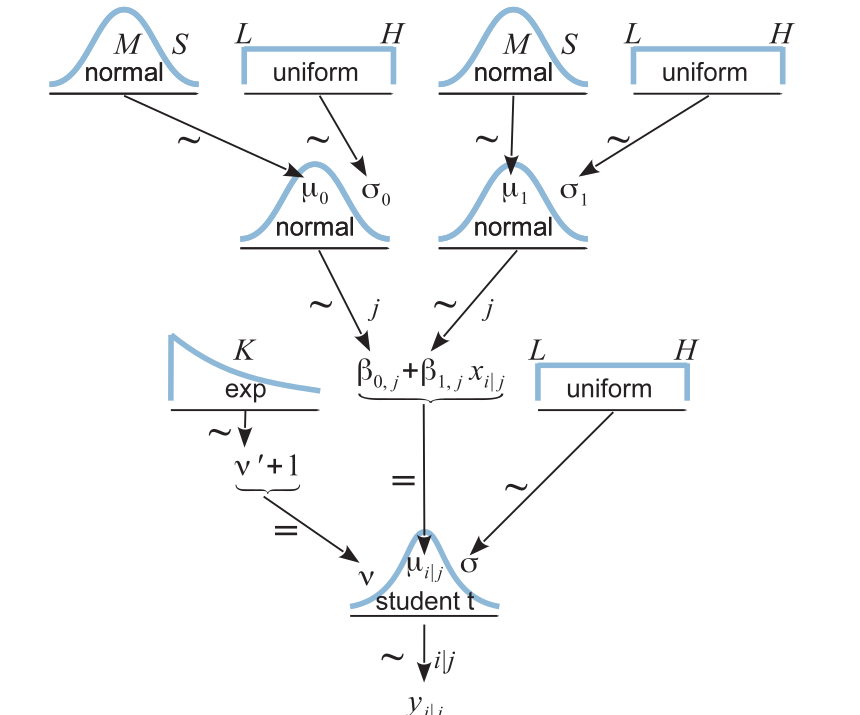
\includegraphics[width=0.8\textwidth]{robust_hierachical_linear_regression}
        \caption{Robust Hierachical Linear Regression Model}
        \label{fig:robust_hierachical_linear_regression}
    \end{figure} 
    \item Mate this is new
\end{itemize}
\end{document}
